\section{Auswertung}
\label{sec:Auswertung}
Vorab: Die Messunsicherheiten wurden gemäß der gaußschen Fehlerfortpflanzung berechnet:
\begin{equation}
  \label{eqn:Gauss}
  \Delta F = \sqrt{\sum_i\left(\frac{\symup{d}F}{\symup{d}y_i}\Delta y_i \right)^2}
\end{equation}

Zuerst wurden alle Gerätekonstanten festgestellt und notiert. Verwendet wurde das Oszilloskop Nummer 4, sowie
die Schaltung Nummer 1. Die Bauteile des Verwendeten Gerätes haben folgende Werte:

\begin{align*}
  &R_1 = (67.2 \pm 0.1) \unit{\ohm} \\
  &R_2 = (682 \pm 0.5) \unit{\ohm}  \\
  &L   = (16.87 \pm 0.05) \unit{\milli\henry} \\
  &C   = (2.060 \pm 0.003) \unit{\nano\farad} \\
\end{align*}

\subsection{Messung zur zeitabhängigkeit der Amplitude}
\label{subsec:AuswertungA}

Um den effektiven Dämpfungswiderstand zu bestimmen verwende man den Zusammenhang \eqref{eqn:def_mu_nu}.
Durch Umstellen auf $R_{\text{eff}}$ ergibt sich die Berechnungsformel:
\begin{equation}
  \label{Abklingdauer1}
  R_{\text{eff}} = 4\pi\mu L
\end{equation}
Um nun $R_{\text{eff}}$ zu berechnen wird zunächst eine Fit-Kurve durch die Messwerte gelegt (siehe \autoref{fig:PlotZuA}).

\begin{table}
  \centering
  \caption{Messdaten zur Zeitabhängigkeit der Amplitude. Abgelesen wurdne die positiven Maxima im Abstand einer Periodendauer.}
  \label{tab:Mess1}
  \begin{tabular}{S[table-format=1.2]}
      \toprule
      $U \mathbin{/} \unit{\volt}$ \\
      \midrule
      3.40 \\
      2.55 \\
      1.95 \\
      1.45 \\
      1.15 \\
      0.85 \\
      0.70 \\
      0.60 \\
      0.50 \\
      0.40 \\
  \bottomrule 
  \end{tabular}
\end{table}

\begin{figure}
  \centering
  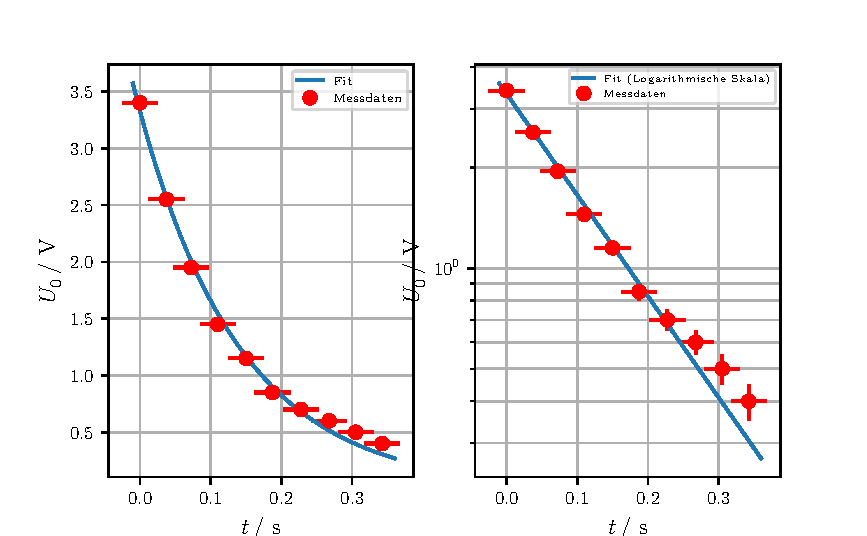
\includegraphics[width=\textwidth]{build/PlotZuA.pdf}
  \caption{Exponentieller Fit \cite{scipy} zu den Messwerten mit linearer Skala (links) und logarithmischer Skala für $U$ (rechts)}
  \label{fig:PlotZuA}
\end{figure}

Man benötigt nun noch den Faktor $2\pi\mu$. Diesen kann man durch die erstellte exponentielle Regression 
bestimmen, da er dem positiven Faktor des Exponenten der Exponentialfunktion entspricht. 
So ist $2\pi\mu = 6.98\, (µs)^{-1}$ gegeben.
$R_{\text{eff}}$ ergibt sich durch einsetzen.

\begin{equation*}
  R_{\text{eff}} = 2\cdot 6.98\cdot 16.87\,\unit{\ohm} = 117.75\,\unit{\ohm}
\end{equation*}

Auffällig ist, dass $R_{\text{eff}} \approx R_1 + 50\unit{\ohm}$ entspricht. Dies hat den Grund, dass der Innenwiderstand des Generators
$50 \unit{\ohm}$ beträgt. Daher wird dieser in den Folgenden Auswertungen berücksichtigt. Unter dieser Voraussetzung beträgt die relative Abweichung des Messwertes
gerade einmal $\Delta R_{\text{rel}} = 0.46\%$.
Die Abklingdauer lässt sich nach Gleichung \eqref{eqn:T_ex} berechnen und ist konkret gegeben durch:
\begin{align*}
  T_{\text{ex, exp}} &= \frac{1}{2\pi\mu} = 143 \unit{\nano\second} \\
  \text{Der Theorie Wert beträgt:} \\
  T_{\text{ex, theo}} &= \frac{2L}{R} = 288 \unit{\nano\second}
\end{align*}

\subsection{Aperiodischer Grenzfall}
\label{subsec:AuswertungB}

Der Theoriewert des Widerstands, bei dem der aperiodische Grenzfall eintritt, lässt sich mit Formel \eqref{eqn:R_ap} berechnen.
Der Fehler dieses Wertes ergibt sich nach der gaußschen Fehlerfortpflanzung \eqref{eqn:Gauss} zu:

\begin{align*}
  \label{eqn:err_R_ap}
  \Delta R_{\text{ap}} &= \sqrt{\Bigl(\frac{\symup{d}R_{\text{ap}}}{\symup{d}L}\Delta L \Bigr)^2+\Bigl(\frac{\symup{d}R_{\text{ap}}}{\symup{d}C}\Delta C\Bigr)^2} \\
  &= \sqrt{\Bigl(\frac{1}{\sqrt{LC}}\Delta L\Bigr)^2+\Bigl(\frac{\sqrt{LC}}{C^2}\Delta C\Bigr)} \\
  &\approx 43 \unit{\ohm}
\end{align*}

Insgesamt erhält man $R_{\text{ap, Theorie}} = (5,72 \pm 0,043) \unit{\kilo\ohm}$. Der experimentell ermittelte Wert wurde 
zu $R_{\text{ap, exp}} = (4,49 \pm 0,01) \unit{\kilo\ohm}$ bestimmt.

\subsection{Frequenzabhängigkeit der Kondensatorspannung}
\label{subsec:AuswertungC}
In \autoref{tab:Mess3} wird das Verhältniss $\frac{U_C}{U}$ gegen die Freuquenz $\nu$ (im Folgenden auch $f$ genannt) aufgetragen. Der Maximalwerte dieses Verhältnisses liegt bei $\nu_{res} \approx 25 \unit{\kilo\hertz}$.
Bei dieser Frequenz ergibt sich für die Resonanzüberhöhung (auch Güte $q$ genannt):
\begin{equation}
  q \pm \Delta q = \frac{U_{C,max}}{U} \pm \sqrt{\frac{\Delta U_{C}}{U_{C}} + \frac{\Delta U}{U}}
  = \left(\frac{9.5\unit{\volt}}{2.8\unit{\volt}} \, \pm \sqrt{\left(\frac{0.05}{11.72}\right)^2 + \left(\frac{0.1}{3}\right)^2}\right)
  = \left(3.39 \pm 0.03\right)
\end{equation}
Der Theoriewert der Güte ergibt sich nach \eqref{eqn:Guete_Resonanzkurve2} zu: $q_{\text{Theorie}} = 3.909$.

\begin{table}
  \centering
  \caption{Frequenzabhängigkeit der Kondensatorspannung $U_c$ und Phase zwischen Erreger- und
   Kondensatorspannung im Serienresonanzkreis. Die Phase $\phi$ wird dabei nach Formel \eqref{eqn:Phase} berechnet}
  \label{tab:Mess3}
  \begin{tabular}{S[table-format=2.1] S[table-format=1.2] S[table-format=1.1] S[table-format=1.2] S[table-format=2.1] S[table-format=3.2] S[table-format=1.2]}
      \toprule
      {$\nu \mathbin{/} \unit{\kilo\hertz}$} & {$U_C \mathbin{/} \unit{\volt}$} & {$U \mathbin{/} \unit{\volt}$} & {$\frac{U_C}{U} \mathbin{/} \unit{\volt}$} &%
      {$a \mathbin{/} \unit{\micro\second}$} & {$b \mathbin{/} \unit{\micro\second}$} & {$\phi \mathbin{/} \unit{\radian}$}\\
      \midrule
      12.5 & 3.10 & 2.9 & 1.07 & 2.5 & 80.0  & 0.20 \\
      15.0 & 3.60 & 3.0 & 1.20 & 2.5 & 66.5  & 0.24 \\
      17.5 & 4.40 & 3.0 & 1.47 & 3.0 & 56.0  & 0.34 \\
      20.0 & 5.40 & 3.0 & 1.80 & 3.5 & 49.5  & 0.44 \\
      22.5 & 7.20 & 2.9 & 2.48 & 5.0 & 44.5  & 0.71 \\
      25.0 & 9.50 & 2.8 & 3.39 & 7.5 & 40.0  & 1.18 \\
      27.5 & 9.00 & 2.8 & 3.21 & 11.0 & 36.0 & 1.92 \\
      30.0 & 6.20 & 2.9 & 2.14 & 12.5 & 33.0 & 2.38 \\
      32.5 & 4.20 & 2.9 & 1.45 & 12.5 & 30.5 & 2.58 \\
      35.0 & 3.10 & 2.9 & 1.07 & 12.0 & 28.5 & 2.65 \\
      37.5 & 2.40 & 2.9 & 0.83 & 11.5 & 26.5 & 2.73 \\
      40.0 & 1.90 & 2.9 & 0.66 & 11.0 & 24.5 & 2.82 \\
      42.5 & 1.55 & 2.9 & 0.53 & 11.0 & 23.5 & 2.94 \\
      45.0 & 1.30 & 2.9 & 0.45 & 10.5 & 22.0 & 3.00 \\
      47.5 & 1.10 & 2.9 & 0.38 & 10.0 & 21.0 & 2.99 \\
      50.0 & 0.95 & 2.9 & 0.33 & 9.5 & 20.0  & 2.98 \\
      52.5 & 0.85 & 2.9 & 0.29 & 9.0 & 19.0  & 2.98 \\
      55.0 & 0.75 & 2.9 & 0.26 & 8.5 & 18.0  & 2.97 \\
      57.5 & 0.70 & 2.9 & 0.24 & 8.0 & 18.0  & 2.79 \\
      \bottomrule
      \end{tabular}
  \end{table}

\begin{figure}
  \centering
  \includegraphics[width=\textwidth]{build/PlotZuC1.pdf}
  \caption{Messwerte im Vergleich zur Theoriekurve, mit halblogarithmischer Skala.}
  \label{fig:PlotZuC1}
\end{figure}

Die Breite der Resonanzkurve $\nu_{\text{diff}}$ kann bestimmt werden durch:
\begin{equation}
  \nu_{\text{diff}} = \nu_+ - \nu_-
\end{equation}
Hierzu werden zunächst die Grenzfrequenzen $\nu_+$ und $\nu_-$ bestimmt. Diese können \autoref{fig:PlotZuC2} entnommen werden.
\begin{equation}
  \nu_+ = 29.37\unit{\kilo\hertz} \,\,\,\,\,\, \nu_- = 22.27\unit{\kilo\hertz} \\
  \rightarrow \nu_{\text{diff}} = 7.1 \unit{\kilo\hertz}
\end{equation}
Die theoretische Resonanzbreite ist nach \eqref{eqn:DeltaOmega} gegeben durch:
\begin{equation}
  \nu_{\text{diff,Theorie}} = \frac{R_2 +50\unit{\ohm}}{2\pi L} = \left(6.91 \pm 0.47\right)\unit{\kilo\hertz}
\end{equation}

\begin{figure}
  \centering
  \includegraphics[width=\textwidth]{build/PlotZuC2.pdf}
  \caption{Breite der Resonanzkurve}
  \label{fig:PlotZuC2}
\end{figure}

\subsection{Frequenzabhängigkeit der Phase zwischen Erreger- und Kondensatorspannung}
\label{subsec:AuswertungD}

Der letzte zu untersuchende Zusammenhang besteht zwischen der Phase $\phi$ und der Generatorfrequenz $\nu$ ($f$). Die ensprechenden Messwerte finden sich
ebenfalls in \autoref{tab:Mess3}. In \autoref{fig:PlotZuD1} ist die Frequenzabhängigkeit der Phase zu erkennen.

\begin{figure}
  \centering
  \includegraphics[width=\textwidth]{build/PlotZuD1.pdf}
  \caption{Messwerte im Vergleich zur Theoriekurve. (halblogarithmische Skala)}
  \label{fig:PlotZuD1}
\end{figure}

\begin{figure}
  \centering
  \includegraphics[width=\textwidth]{build/PlotZuD2.pdf}
  \caption{Die Frequenzen $f_1$ ($\nu_1$) und $f_2$ ($\nu_2$) lassen sich gut am Graphen der Messwerte ablesen. (Skala linear)}
  \label{fig:PlotZuD2}
\end{figure}

In \autoref{fig:PlotZuD2} sind die experimentell ermittelten Frequenzen $\nu_1 = 22.9 \, \symup{kHz}$ und \\ $\nu_2 = 29.8 \, \symup{kHz}$ eingezeichnet.
Die Theoriewerte ergeben sich nach \eqref{eqn:w_1_w_2} unter berücksichtigung der gaußschen Fehlerfortpflanzung \eqref{eqn:Gauss} zu:

\begin{align*}
  \nu_{1,\text{Theorie}} &= (23.54 \pm 0.04) \symup{kHz} \\
  \nu_{2,\text{Theorie}} &= (30.45 \pm 0.05) \symup{kHz}
\end{align*}

\cite{uncertainties}

